\documentclass[10pt,twocolumn]{article}

\usepackage[T1]{fontenc}
\usepackage{lmodern}
\usepackage[letterpaper,margin=0.70in,columnsep=0.25in]{geometry}
\usepackage{amsmath,amssymb}
\usepackage{booktabs}
\usepackage{array}
\usepackage{graphicx}
\usepackage{xcolor}
\usepackage{caption}
\usepackage{enumitem}
\usepackage{siunitx}
\usepackage{tikz}
\usepackage{hyperref}
\usepackage{cleveref}
\usepackage{placeins}

\usetikzlibrary{arrows.meta,positioning,fit,calc}
\graphicspath{{figures/}}
\sisetup{detect-all,round-mode=places,round-precision=3}
\setlist{nosep,leftmargin=*}
\captionsetup{font=small,labelfont=bf}

\definecolor{egfnblue}{HTML}{2878B5}
\definecolor{egfnorange}{HTML}{E07B39}
\definecolor{egfngreen}{HTML}{3A9D5D}
\definecolor{egfnpurple}{HTML}{7A5195}
\definecolor{softgray}{HTML}{F2F4F5}

\hypersetup{
  colorlinks=true,
  linkcolor=egfnblue,
  citecolor=egfngreen,
  urlcolor=egfnorange,
  pdftitle={Energy-Gated Frequency Networks},
  pdfauthor={Henry}
}

\newcommand{\egfn}{EGFN}
\newcommand{\vect}[1]{\boldsymbol{#1}}

\tikzset{
  block/.style={draw,rounded corners=2pt,minimum height=8mm,align=center,
    font=\footnotesize,inner xsep=5pt},
  flow/.style={-{Latex[length=2mm]},thick},
  tensor/.style={font=\scriptsize,text=black!70}
}

\title{\vspace{-1.2em}\textbf{Energy-Gated Frequency Networks}}
\author{Henry\\Independent Research and Portfolio Project}
\date{July 2026}

\begin{document}
\raggedbottom

\twocolumn[
\maketitle
\vspace{-1.6em}
\begin{center}
\begin{minipage}{0.93\textwidth}
\textbf{Abstract.}
This work investigates whether low-pass, high-pass, and band-pass filtering can
be embedded in a neural network so that energy in specific spectral regions
modulates the activations used for audio classification. We introduce the
Energy-Gated Frequency Network (\egfn), a raw-waveform architecture that
exposes per-band filter responses, energy, and learned gates before temporal
classification. The study progresses from controlled sinusoids to spoken
digits, keyword spotting, and industrial valve anomaly detection. Free FIR
kernels improve flexibility while losing their original physical band
interpretation; Sinc-parameterized filters preserve explicit cutoffs but reduce
performance in the controlled screening experiment. In a preliminary
three-seed MIMII Valve comparison, a wide \egfn{} produced higher calibrated F1
than a smaller Conv1D baseline, although the architectures were not capacity
matched. In a separate single-seed capacity-matched screening experiment,
Conv1D achieved higher F1, while free-filter \egfn{} retained a small ROC--AUC
advantage. These results are descriptive and do not establish statistical
superiority. \egfn{} is therefore presented as a frequency-structured research
architecture for studying spectral energy, adaptive modulation, and the
trade-off between physical interpretability and predictive flexibility.

\vspace{0.45em}
\textbf{Keywords:} raw audio, learnable filter bank, energy gating,
interpretability, keyword spotting, industrial anomaly detection.
\end{minipage}
\end{center}
\vspace{1.0em}
]

\section{Introduction}

Audio classifiers based on one-dimensional convolution can learn effective
waveform representations directly from data. Their first-layer kernels can be
interpreted as filters, but standard training does not require those kernels to
remain low-pass, high-pass, or band-pass systems. This project began with a
physical question: if classical filters separate sinusoidal components in
electrical and digital signals, can the same principle organize neural
activation for audio classification?

The central research question is:

\begin{quote}
Can low-pass, high-pass, and band-pass filtering be embedded within a neural
network so that energy in specific spectral regions selectively controls the
activations used for audio classification?
\end{quote}

The goal is not to announce a universally superior architecture. The goal is
to answer the question through progressively harder experiments, including
negative and ambiguous results. The paper follows the concise progression from
mechanism to controlled evaluation used in modern architecture papers such as
Vaswani et al.~\cite{vaswani2017attention}, without implying any architectural
relationship to the Transformer.

The main contributions are:

\begin{enumerate}
  \item a differentiable frequency--energy--gate block for raw waveforms;
  \item visual evidence of how band energy and gates respond to input
        frequency and task difficulty;
  \item experiments across synthetic signals, FSDD, Speech Commands, and MIMII;
  \item a three-seed industrial comparison followed by a capacity-matched
        control;
  \item an explicit analysis of observability, physical interpretability, and
        parameter efficiency.
\end{enumerate}

\section{Background and Motivation}

\subsection{From neurons to waveform classifiers}

A feed-forward neural network transforms an input $\vect{x}$ through hidden
layers and produces output logits:
\begin{align}
  \vect{h}^{(\ell)}
  &=\phi\!\left(W^{(\ell)}\vect{h}^{(\ell-1)}+\vect{b}^{(\ell)}\right),\\
  \vect{o}&=W^{(L)}\vect{h}^{(L-1)}+\vect{b}^{(L)}.
\end{align}
The input contains observations, hidden layers construct task-relevant
representations, and the output scores are converted into class probabilities.
Nonlinear activations prevent the entire stack from collapsing into a single
linear transformation~\cite{lecun2015deep}.

For mono audio, the input is a sampled sequence
$x[n]$ represented as $\vect{x}\in\mathbb{R}^{B\times1\times T}$. A Conv1D
layer applies learned finite kernels:
\begin{equation}
  u_k[n]=\sum_{m=0}^{K-1}h_k[m]x[n-m].
  \label{eq:conv}
\end{equation}
Thus Conv1D already performs learned filtering. The distinction in this work is
not ``filtering versus convolution,'' but whether frequency structure, energy,
and modulation are explicitly parameterized and exposed.

\subsection{Structured learnable audio frontends}

SincNet learns only low and high cutoff frequencies of first-layer band-pass
filters~\cite{ravanelli2018sincnet}. LEAF extends learnable audio frontends with
filtering, pooling, compression, and normalization~\cite{zeghidour2021leaf}.
These works motivate a useful middle ground between fixed signal-processing
features and unconstrained convolution. \egfn{} explores a related but distinct
question: can explicit per-band energy drive a learned multiplicative gate, and
what does that gate reveal about model behavior?

The Sinc mode evaluated here is a Sinc-parameterized frontend, not a complete
reimplementation of SincNet. Likewise, LEAF contains additional learnable
pooling, compression, and normalization components. No direct SincNet or LEAF
baseline is reported; this limits claims about novelty relative to established
learnable frontends.

\section{Energy-Gated Frequency Network}

\subsection{Filter-bank frontend}

The frontend receives $\vect{x}\in\mathbb{R}^{B\times1\times T}$ and produces
$M$ aligned band responses. For an odd kernel length $K=101$, a windowed
low-pass response is initialized as
\begin{equation}
  h_{\mathrm{LP}}[n;f_c]
  =2\frac{f_c}{f_s}\,
   \operatorname{sinc}\!\left(2\frac{f_c}{f_s}n\right)w[n],
  \label{eq:lowpass}
\end{equation}
where $w[n]$ is a Hamming window for the fixed and free modes. High-pass and
band-pass filters follow from spectral inversion and subtraction:
\begin{align}
  h_{\mathrm{HP}}[n;f_c] &= \delta[n]-h_{\mathrm{LP}}[n;f_c],\\
  h_{\mathrm{BP}}[n;f_l,f_h] &= h_{\mathrm{LP}}[n;f_h]-h_{\mathrm{LP}}[n;f_l].
\end{align}

Three modes were evaluated:
\begin{itemize}
  \item \textbf{Fixed:} initialized FIR coefficients remain constant.
  \item \textbf{Free:} every FIR coefficient becomes trainable.
  \item \textbf{Sinc:} only ordered low and high cutoffs are learned, while a
        Hann-windowed band-pass kernel is reconstructed during each forward
        pass.
\end{itemize}

The eight-band fine initialization is
$<250$, $250$--$500$, $500$--$750$, $750$--$1000$,
$1000$--$1500$, $1500$--$2500$, $2500$--$4000$, and $>4000$ Hz.
In free mode these names describe initialization only; they do not guarantee
the learned spectral support.

\subsection{Energy-dependent gating}

After filtering, bias and GELU activation are applied:
\begin{align}
  u_k[n] &= (h_k*x)[n],\\
  a_k[n] &= \operatorname{GELU}(u_k[n]+b_k).
\end{align}
The mean-square energy of each unactivated response is
\begin{equation}
  E_k=\frac{1}{T}\sum_{n=1}^{T}u_k[n]^2.
  \label{eq:energy}
\end{equation}
For independent gates,
\begin{equation}
  g_k=\sigma\!\left(\alpha_k\log(1+E_k)+\beta_k\right),
  \label{eq:gate}
\end{equation}
and the output is
\begin{equation}
  y_k[n]=g_k a_k[n].
  \label{eq:output}
\end{equation}
A contextual alternative predicts all gates from the complete log-energy
vector, $\vect{g}=\sigma(\operatorname{MLP}(\log(1+\vect{E})))$.

\begin{figure*}[t]
\centering
\resizebox{0.98\textwidth}{!}{%
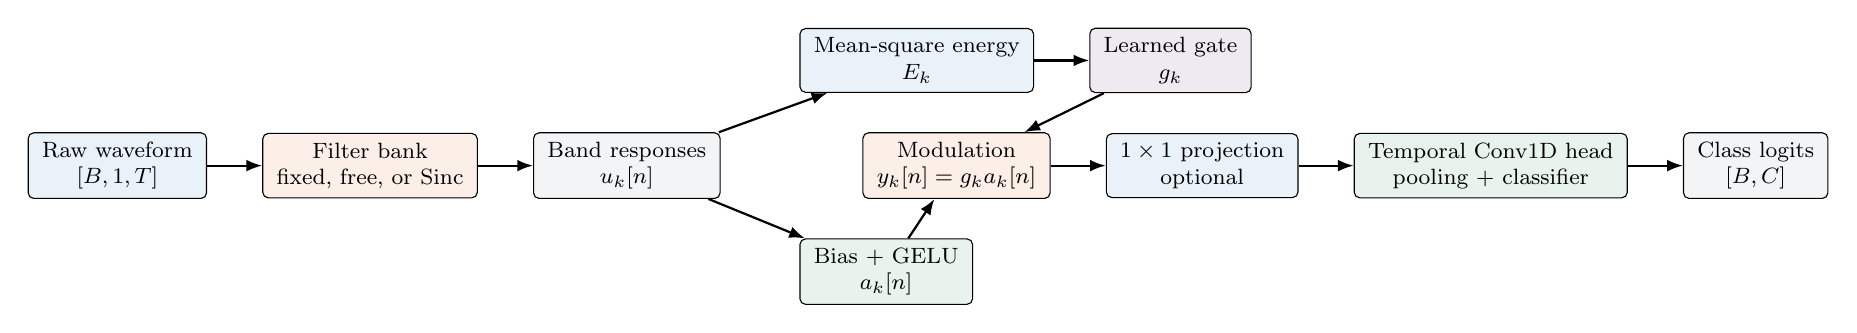
\begin{tikzpicture}[node distance=7mm and 7mm]
  \node[block,fill=egfnblue!10] (input) {Raw waveform\\$[B,1,T]$};
  \node[block,fill=egfnorange!12,right=of input] (filters) {Filter bank\\fixed, free, or Sinc};
  \node[block,fill=softgray,right=of filters] (response) {Band responses\\$u_k[n]$};
  \node[block,fill=egfnblue!10,above right=5mm and 10mm of response] (energy) {Mean-square energy\\$E_k$};
  \node[block,fill=egfnpurple!12,right=of energy] (gate) {Learned gate\\$g_k$};
  \node[block,fill=egfngreen!12,below right=5mm and 10mm of response] (activation) {Bias + GELU\\$a_k[n]$};
  \node[block,fill=egfnorange!12,right=18mm of response] (multiply) {Modulation\\$y_k[n]=g_ka_k[n]$};
  \node[block,fill=egfnblue!10,right=of multiply] (projection) {$1\times1$ projection\\optional};
  \node[block,fill=egfngreen!12,right=of projection] (temporal) {Temporal Conv1D head\\pooling + classifier};
  \node[block,fill=softgray,right=of temporal] (logits) {Class logits\\$[B,C]$};
  \draw[flow] (input) -- (filters);
  \draw[flow] (filters) -- (response);
  \draw[flow] (response) -- (energy);
  \draw[flow] (energy) -- (gate);
  \draw[flow] (response) -- (activation);
  \draw[flow] (gate) -- (multiply);
  \draw[flow] (activation) -- (multiply);
  \draw[flow] (multiply) -- (projection);
  \draw[flow] (projection) -- (temporal);
  \draw[flow] (temporal) -- (logits);
\end{tikzpicture}}
\caption{Complete Temporal \egfn{} flow. Unlike a standard Conv1D frontend,
the model explicitly exposes band responses, mean-square energy, and
multiplicative gates. The downstream temporal head retains ordering that the
initial pooled classifier discarded.}
\label{fig:architecture}
\end{figure*}
\FloatBarrier

\subsection{Classifier evolution}

The initial classifier pooled each band using mean, maximum, standard
deviation, log-energy, and gate values before a small MLP. This representation
was compact and interpretable, but global pooling removed temporal ordering.
Temporal \egfn{} therefore sends the gated sequences through a lightweight
Conv1D head. The wide configuration adds an $8\!\rightarrow\!32$ pointwise
projection followed by $64$- and $128$-channel temporal blocks.

\section{Hypotheses and Experimental Design}

Five initial hypotheses guided the work:
\begin{description}[style=nextline]
  \item[H1: Frequency decomposition.] Band outputs should respond most strongly
  near their designed spectral regions.
  \item[H2: Energy-dependent modulation.] Gates should change as band energy
  changes.
  \item[H3: Predictive utility.] The frontend should support competitive audio
  classification.
  \item[H4: Observability.] Energy, gates, and filter responses should make
  internal behavior inspectable.
  \item[H5: Adaptation.] Learnable filters should improve difficult tasks, even
  if unconstrained learning weakens physical interpretation.
\end{description}

The experimental narrative follows the same sequence throughout:
\emph{problem $\rightarrow$ architectural change $\rightarrow$ hypothesis
$\rightarrow$ experiment $\rightarrow$ visualization $\rightarrow$ revised
question}. Models were implemented in PyTorch~\cite{paszke2019pytorch}.

\begin{table}[t]
\centering
\caption{Real-audio datasets and evaluated task.}
\label{tab:datasets}
\small
\begin{tabular}{@{}lll@{}}
\toprule
Dataset & Task & Split focus \\
\midrule
FSDD~\cite{jackson2016fsdd} & 10 digits & random / speaker \\
Speech Commands~\cite{warden2018speech} & 10 keywords & official \\
MIMII~\cite{purohit2019mimii} & valve anomaly & stratified \\
\bottomrule
\end{tabular}
\end{table}

Accuracy is reported for balanced multiclass tasks. For MIMII, where normal
recordings dominate, precision, recall, F1, and ROC-AUC are emphasized.
Classification thresholds are selected on validation by maximizing F1 and are
then frozen for test evaluation.

\section{Synthetic Proof of Mechanism}

\subsection{Frequency response of the first prototype}

The first model used five fixed filters and independent gates. A constant-RMS
sinusoid was swept from $50$ to $7950$ Hz in $25$ Hz increments and averaged
over four phases. 

\begin{figure*}[t]
\centering
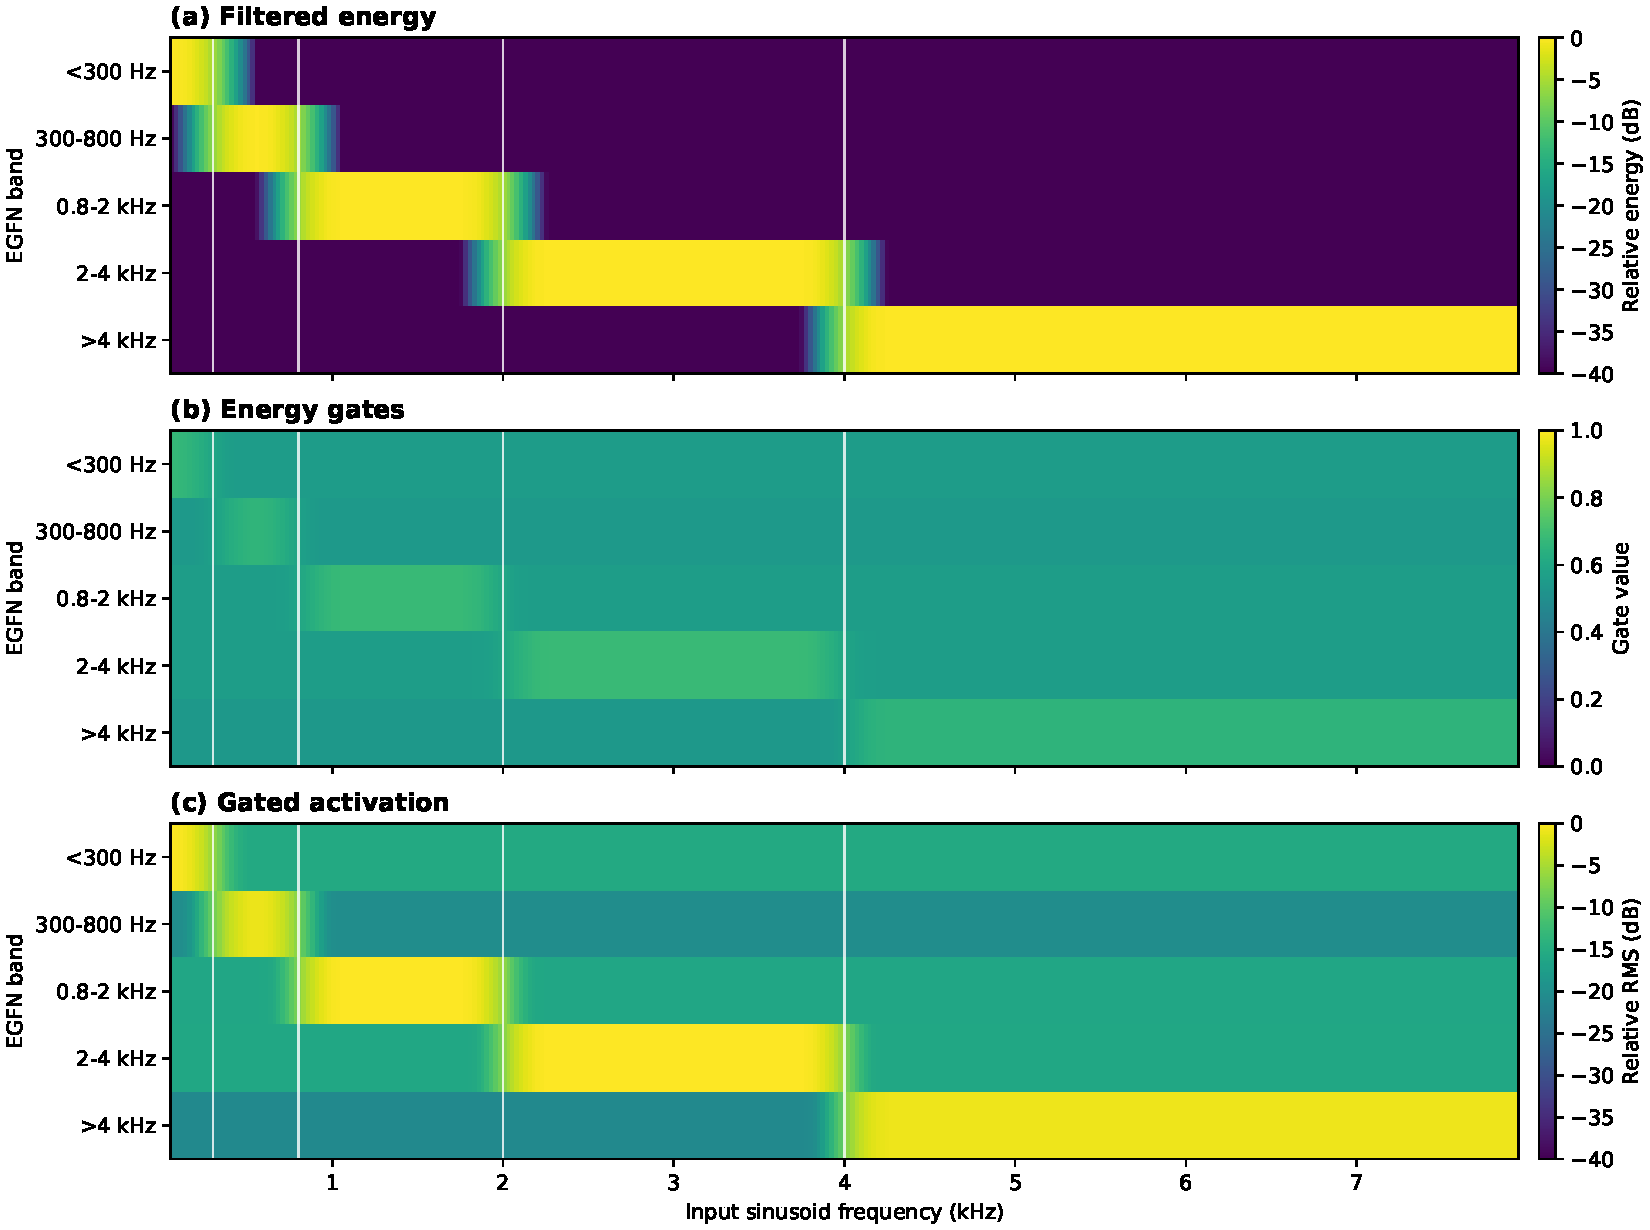
\includegraphics[width=0.98\textwidth]{fig01_frequency_sweep.pdf}
\caption{Sinusoidal activation sweep for the V0 checkpoint. Energy follows the
expected coarse bands, while gates remain soft rather than binary. The figure
validates frequency-dependent observability, not hard band selection.}
\label{fig:v0sweep}
\end{figure*}

\Cref{fig:v0sweep} supports H1: energy tracks the filter-bank structure. The
gates range approximately from $0.533$ to $0.677$, supporting energy-dependent
modulation but not discrete selection. Residual activation outside the nominal
passband is expected from finite FIR responses, bias, and GELU.

\subsection{Easy versus hard synthetic classes}

The same checkpoint was evaluated without retraining on $2048$ unseen easy and
$2048$ hard examples at 15 dB SNR. Easy classes occupied separated frequency
regions; hard classes overlapped primarily between roughly $400$ and $1500$ Hz.

\begin{figure*}[t]
\centering
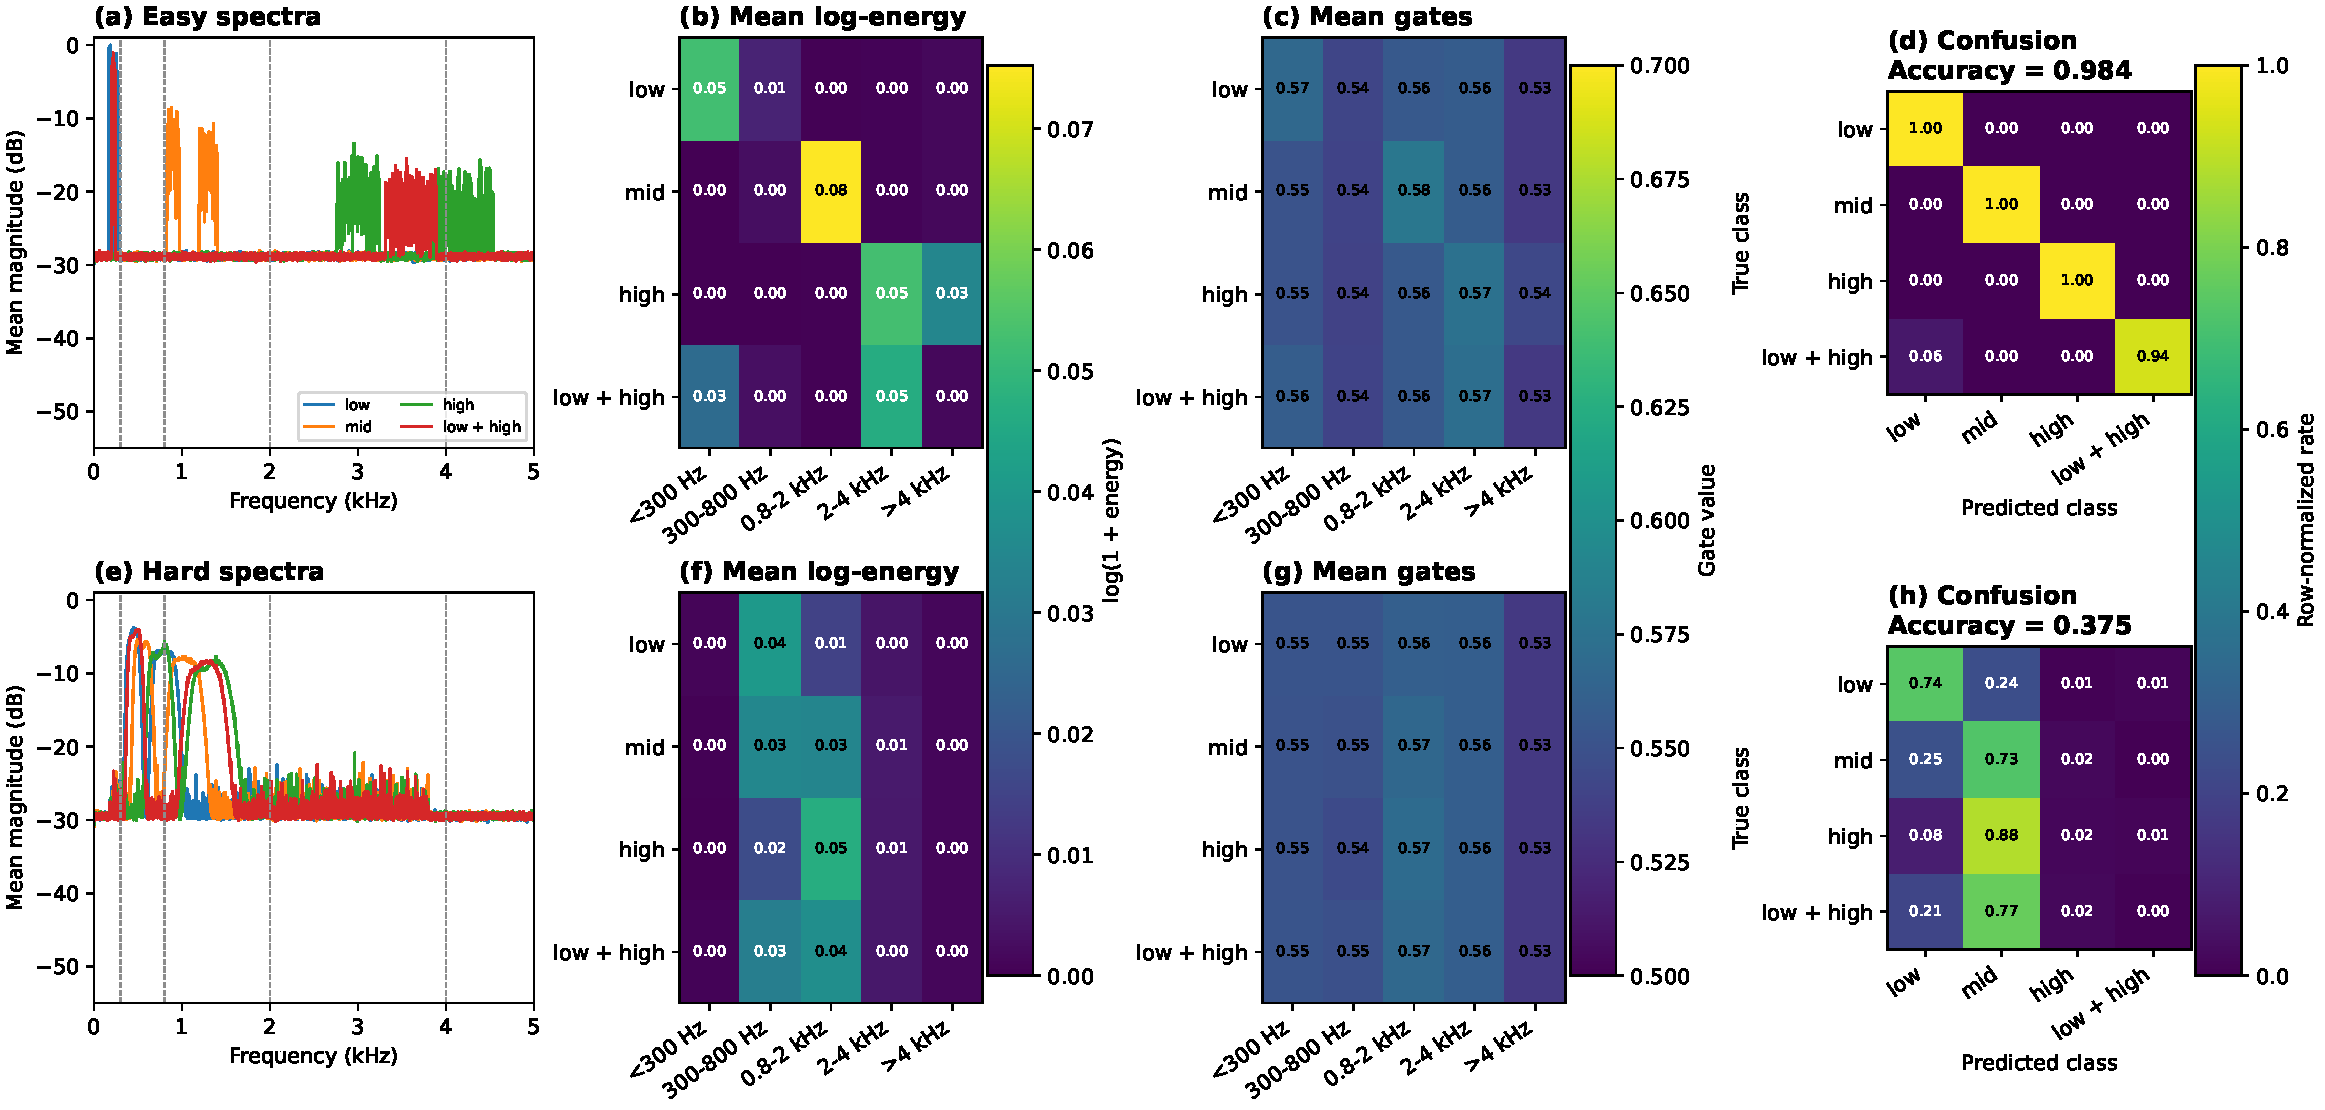
\includegraphics[width=0.98\textwidth]{fig02_easy_vs_hard.pdf}
\caption{Behavior of one V0 checkpoint on easy and hard synthetic data. Test
accuracy falls from $0.984$ to $0.375$ when class spectra overlap. The filters
still respond, but the coarse representation no longer separates the labels.}
\label{fig:easyhard}
\end{figure*}

The failure in \cref{fig:easyhard} was informative: correct filtering does not
guarantee sufficient class resolution. It motivated a finer eight-band bank
and learnable filters.

\subsection{Compact architecture progression}

\Cref{tab:syntheticprogression} summarizes the remaining synthetic iterations.
Increasing frequency resolution and freeing the FIR coefficients improved the
hard task, but free kernels became irregular and multi-band. Independent and
contextual gates reached the same best validation accuracy. Sparsity
regularization produced the highest value in this small experiment, although
the gates remained soft rather than binary. Detailed filter sweeps and gate
distributions are provided in the supplementary material.

\begin{table}[t]
\centering
\caption{Synthetic hard-task progression. Results are best validation
accuracies from the corresponding development runs.}
\label{tab:syntheticprogression}
\small
\begin{tabular}{@{}llr@{}}
\toprule
Frontend & Gate configuration & Best val. \\
\midrule
Five-band fixed & independent & 0.531 \\
Eight-band fixed & independent & 0.633 \\
Eight-band free FIR & independent & 0.703 \\
Eight-band free FIR & contextual & 0.703 \\
Eight-band free FIR & sparse penalty & \textbf{0.727} \\
\bottomrule
\end{tabular}
\end{table}

These runs do not isolate the contribution of gating because every row retains
an energy gate. Consequently, they establish architectural progression but not
that gating outperforms an otherwise identical ungated filter bank.
\FloatBarrier

\section{From Synthetic Signals to Speech}

\subsection{FSDD: split and temporal structure}

FSDD contains $3000$ recordings of ten English digits from six speakers in the
version used here~\cite{jackson2016fsdd}. A random recording split yielded test
accuracy $0.840$, but the same pooled \egfn{} fell to $0.560$ when the test
speaker was unseen. The random result is valid for its protocol, but cannot
demonstrate speaker invariance. Replacing global pooling with a temporal head
raised speaker-disjoint test accuracy to $0.708$; Conv1D reached $0.746$.

\begin{table}[t]
\centering
\caption{FSDD speaker-disjoint results.}
\label{tab:fsddtemporal}
\small
\begin{tabular}{@{}lrrr@{}}
\toprule
Model & Params. & Best val. & Test \\
\midrule
Pooled \egfn{} & 4,106 & 0.538 & 0.560 \\
Temporal \egfn{} & 44,714 & \textbf{0.724} & 0.708 \\
Conv1D & 27,594 & 0.704 & \textbf{0.746} \\
\bottomrule
\end{tabular}
\end{table}

This stage demonstrates the importance of temporal structure, not an isolated
advantage of the frequency frontend. Training histories and confusion matrices
for both split protocols are retained in the supplementary material.

\subsection{Scaling to Speech Commands}

Speech Commands is designed for reproducible limited-vocabulary keyword
spotting~\cite{warden2018speech}. Ten commands were used with the official
train/validation/test split: $30{,}769/3{,}703/4{,}074$ recordings. Training
included waveform augmentation.

\begin{figure*}[t]
\centering
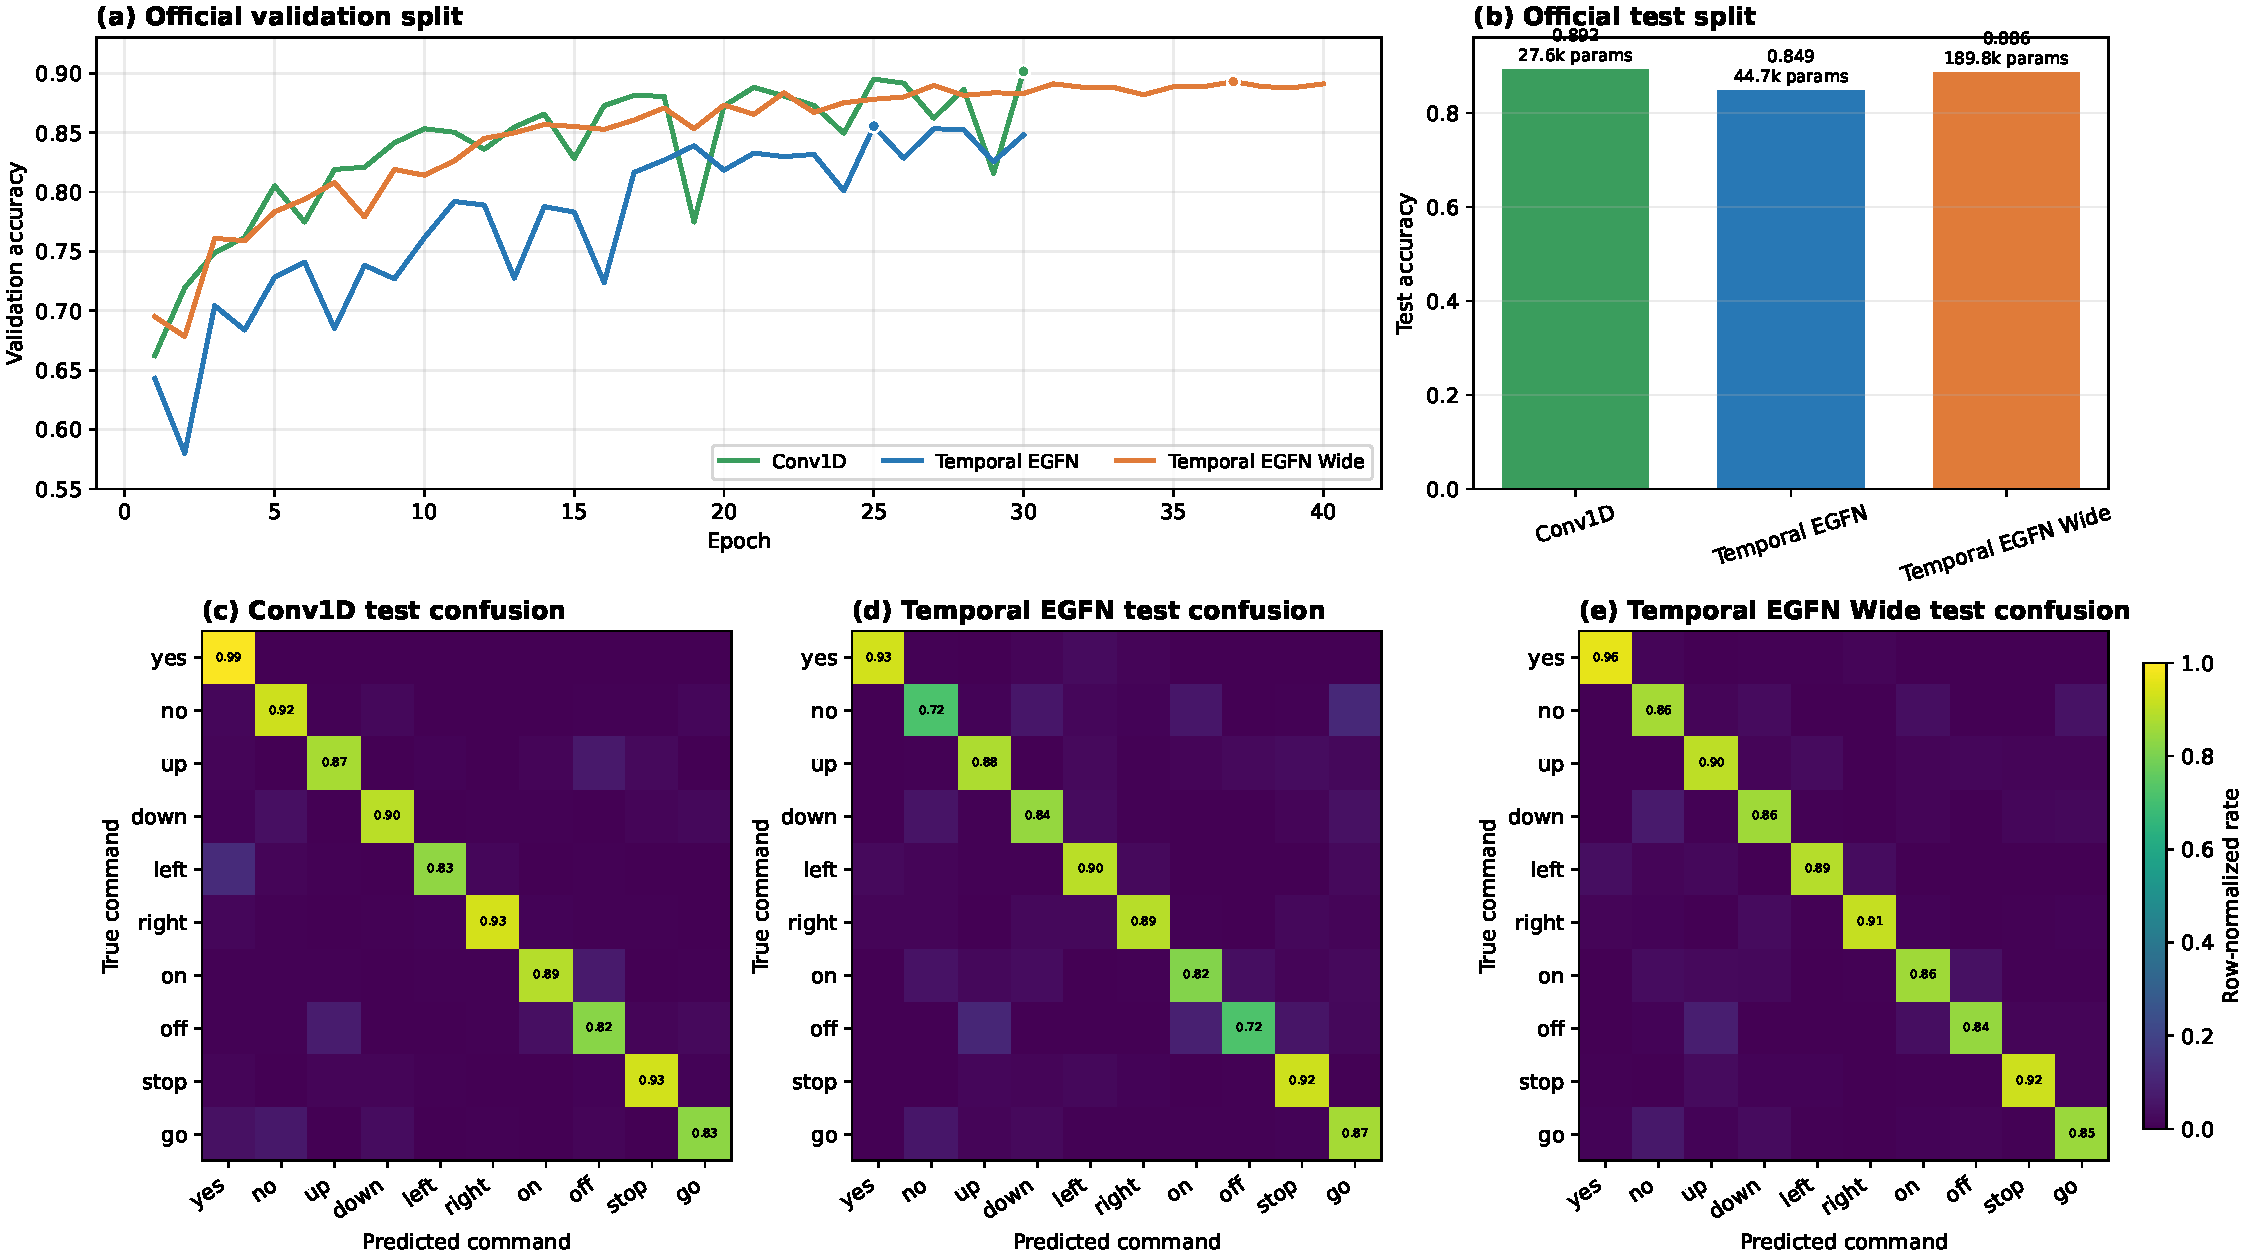
\includegraphics[width=0.98\textwidth]{fig07_speech_commands.pdf}
\caption{Speech Commands results. Temporal \egfn{} Wide reaches test accuracy
$0.886$, close to Conv1D at $0.892$, and improves several class recalls. The
near match requires substantially more parameters.}
\label{fig:speechcommands}
\end{figure*}
\FloatBarrier

\begin{table}[t]
\centering
\caption{Speech Commands comparison.}
\label{tab:speech}
\small
\begin{tabular}{@{}lrrr@{}}
\toprule
Model & Params. & Best val. & Test \\
\midrule
Conv1D & 27,594 & \textbf{0.902} & \textbf{0.892} \\
Temporal \egfn{} & 44,714 & 0.856 & 0.849 \\
Temporal \egfn{} Wide & 189,802 & 0.893 & 0.886 \\
\bottomrule
\end{tabular}
\end{table}

The wide model reduces the accuracy gap to $0.0066$, showing that its
frequency-gated representation can support competitive classification.
However, it uses approximately $6.9$ times the parameters of this Conv1D
baseline. The result supports viability, not parameter efficiency.

\section{Industrial Anomaly Detection}

\subsection{Why machinery is a relevant domain}

MIMII contains normal and anomalous sounds from industrial machines, including
valves, pumps, fans, and slide rails~\cite{purohit2019mimii}. Mechanical faults
can alter rotational components, harmonics, broadband friction, leakage, and
high-frequency impacts. This makes machinery a stronger physical test of a
frequency-structured frontend than spoken-word identity alone.

The valve subset used here contains $4170$ recordings, split into
$2922/624/624$ train/validation/test examples. The test set contains $553$
normal and $71$ anomalous recordings. Balanced cross-entropy, augmentation,
label smoothing, cosine scheduling, and early stopping were used.

\subsection{Initial seed-42 application}

The initial comparison used the original small Conv1D and Temporal \egfn{}
Wide. Thresholds were selected on validation and applied once to test.

\begin{figure*}[t]
\centering
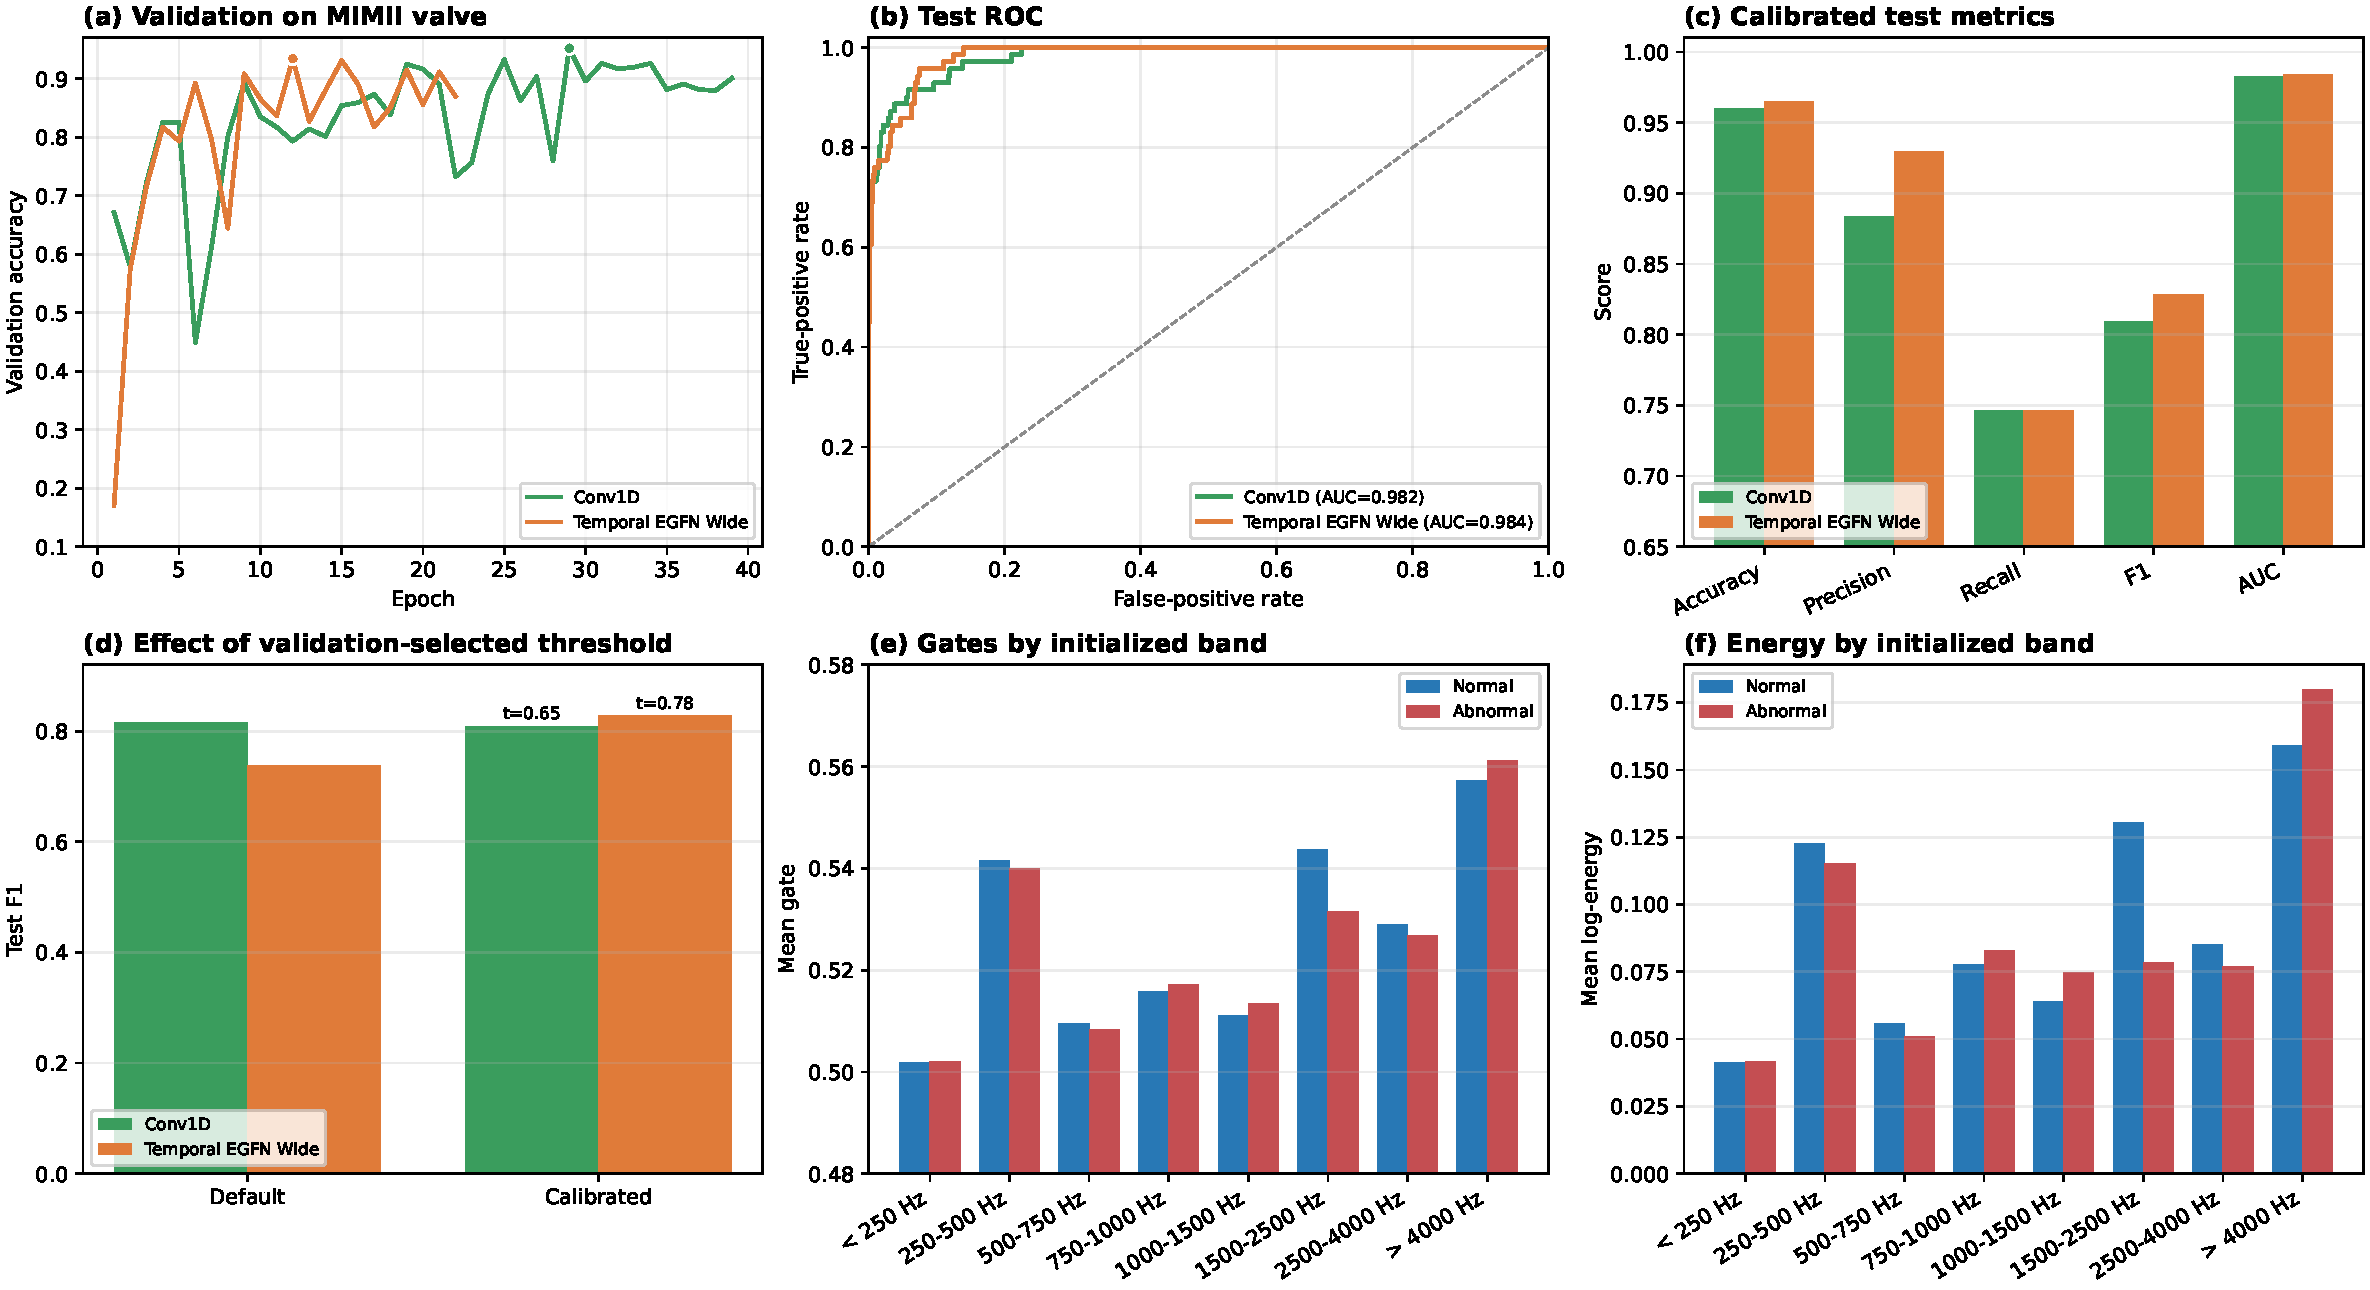
\includegraphics[width=0.98\textwidth]{fig08_mimii_initial.pdf}
\caption{Initial MIMII Valve application. At validation-selected thresholds,
\egfn{} reaches F1 $0.828$ and AUC $0.984$, versus F1 $0.809$ and AUC $0.982$
for Conv1D. Energy differences are more pronounced than gate differences.}
\label{fig:mimiiinitial}
\end{figure*}

Calibration reduced \egfn{} false positives from $35$ to $4$, while recall
decreased from $0.873$ to $0.746$. The strongest energy differences appeared
above $4$ kHz and in the initialized $1.5$--$2.5$ kHz channel. Gate differences
between normal and abnormal recordings remained small, with maximum magnitude
near $0.012$. Thus the model exposes useful internal measurements, but its gates
are not class-specific switches.

\subsection{Three-seed experiment}

Seeds $42$, $123$, and $456$ used the same protocol. Each run selected its
threshold using validation only. With only three seeds, the mean and sample
standard deviation below are descriptive summaries, not confidence intervals
or evidence of statistical significance.

\begin{figure*}[t]
\centering
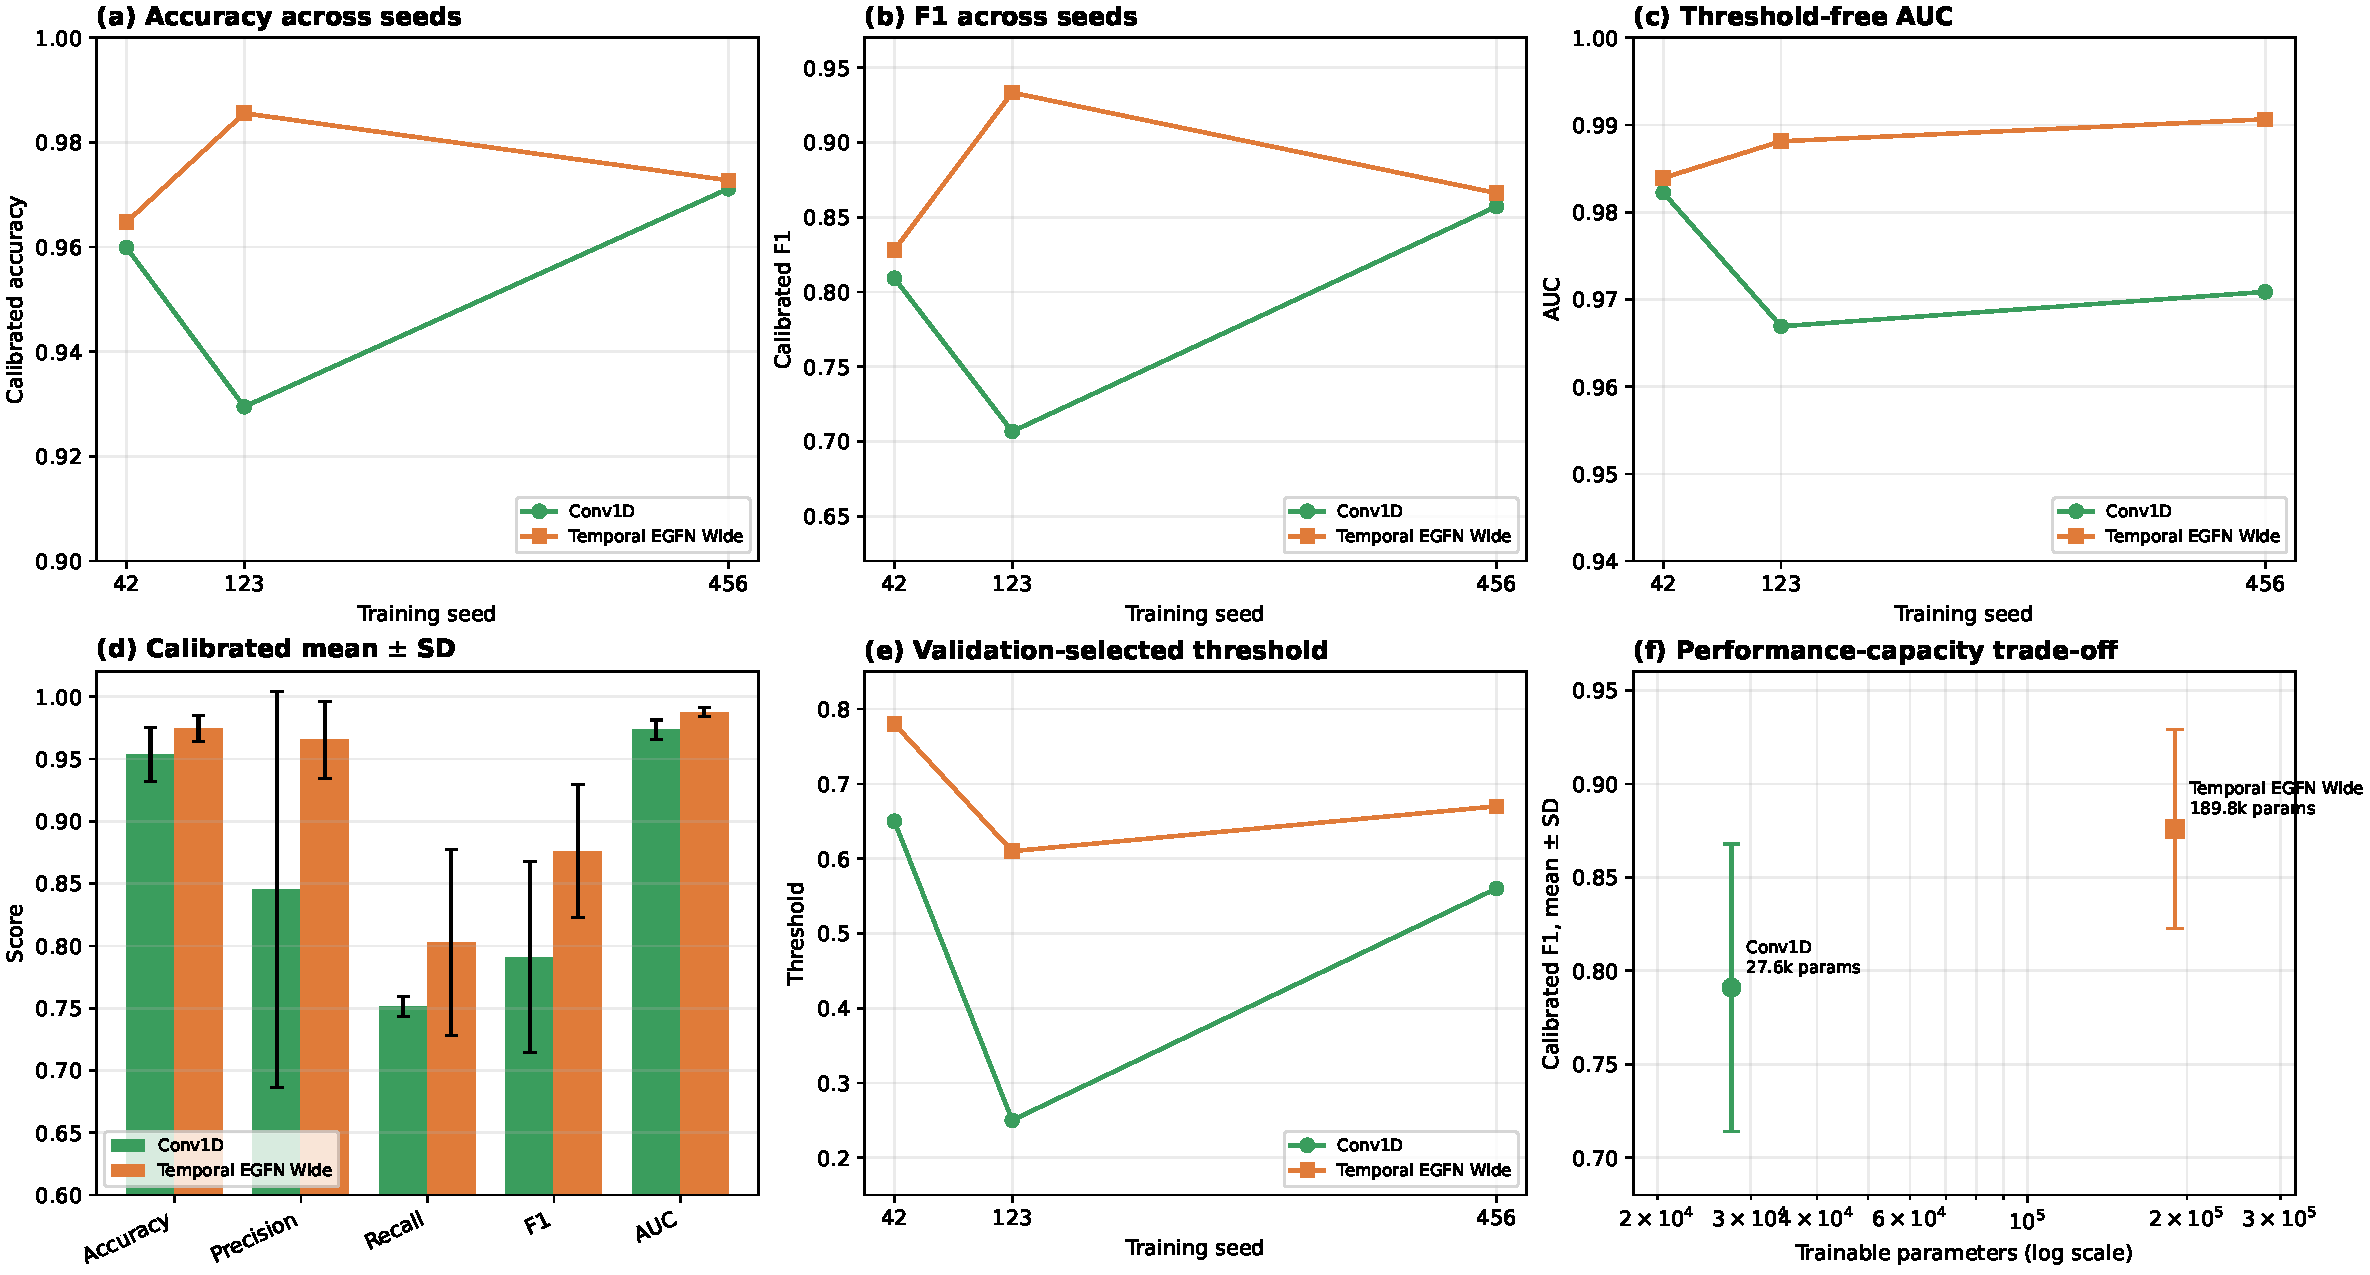
\includegraphics[width=0.98\textwidth]{fig09_mimii_multiseed.pdf}
\caption{Preliminary three-seed MIMII comparison. Temporal \egfn{} Wide is
higher in calibrated accuracy, F1, and AUC for these three runs. The
performance--capacity panel also exposes the $6.9\times$ parameter gap.}
\label{fig:mimiimultiseed}
\end{figure*}
\FloatBarrier

\begin{table}[t]
\centering
\caption{Descriptive MIMII mean $\pm$ sample standard deviation for three
seeds; no significance claim is made.}
\label{tab:multiseed}
\small
\resizebox{\columnwidth}{!}{%
\begin{tabular}{@{}lccc@{}}
\toprule
Model & Accuracy & F1 & AUC \\
\midrule
Conv1D & $0.954\pm0.022$ & $0.791\pm0.077$ & $0.973\pm0.008$ \\
\egfn{} Wide & $\mathbf{0.974\pm0.011}$ & $\mathbf{0.876\pm0.053}$ & $\mathbf{0.988\pm0.003}$ \\
\bottomrule
\end{tabular}
}
\end{table}

The architectures are not capacity matched. The experiment therefore raises
rather than resolves the attribution question: does \egfn{} improve because of
its frontend or because its temporal model is larger?

\section{Controlled V2 Frontend Study}

\subsection{Capacity-matched protocol}

The final control fixes eight frontend channels, the $8\!\rightarrow\!32$
projection, the $64/128$ temporal head, classifier, augmentation, loss,
regularization, split, and seed. Only the frontend changes:

\begin{table}[t]
\centering
\caption{V2 controlled architectures.}
\label{tab:v2params}
\small
\begin{tabular}{@{}llr@{}}
\toprule
Experiment & Frontend & Parameters \\
\midrule
Matched Conv1D & free waveform conv. & 188,754 \\
\egfn{}-Free & free FIR + energy/gates & 188,770 \\
\egfn{}-Sinc & learned cutoffs + gates & 187,978 \\
\bottomrule
\end{tabular}
\end{table}

The free Conv1D and \egfn{} differ by only $16$ parameters. In Sinc mode,
sigmoid-parameterized lower cutoffs and positive bandwidths guarantee ordered
cutoffs, at least $50$ Hz bandwidth, and an upper cutoff below Nyquist.
This control still compares only gated \egfn{} variants; it does not isolate
gating from the filter bank itself. An ungated matched protocol is specified in
the repository but is not reported because those runs were not yet completed.

\subsection{Controlled result}

\begin{figure*}[t]
\centering
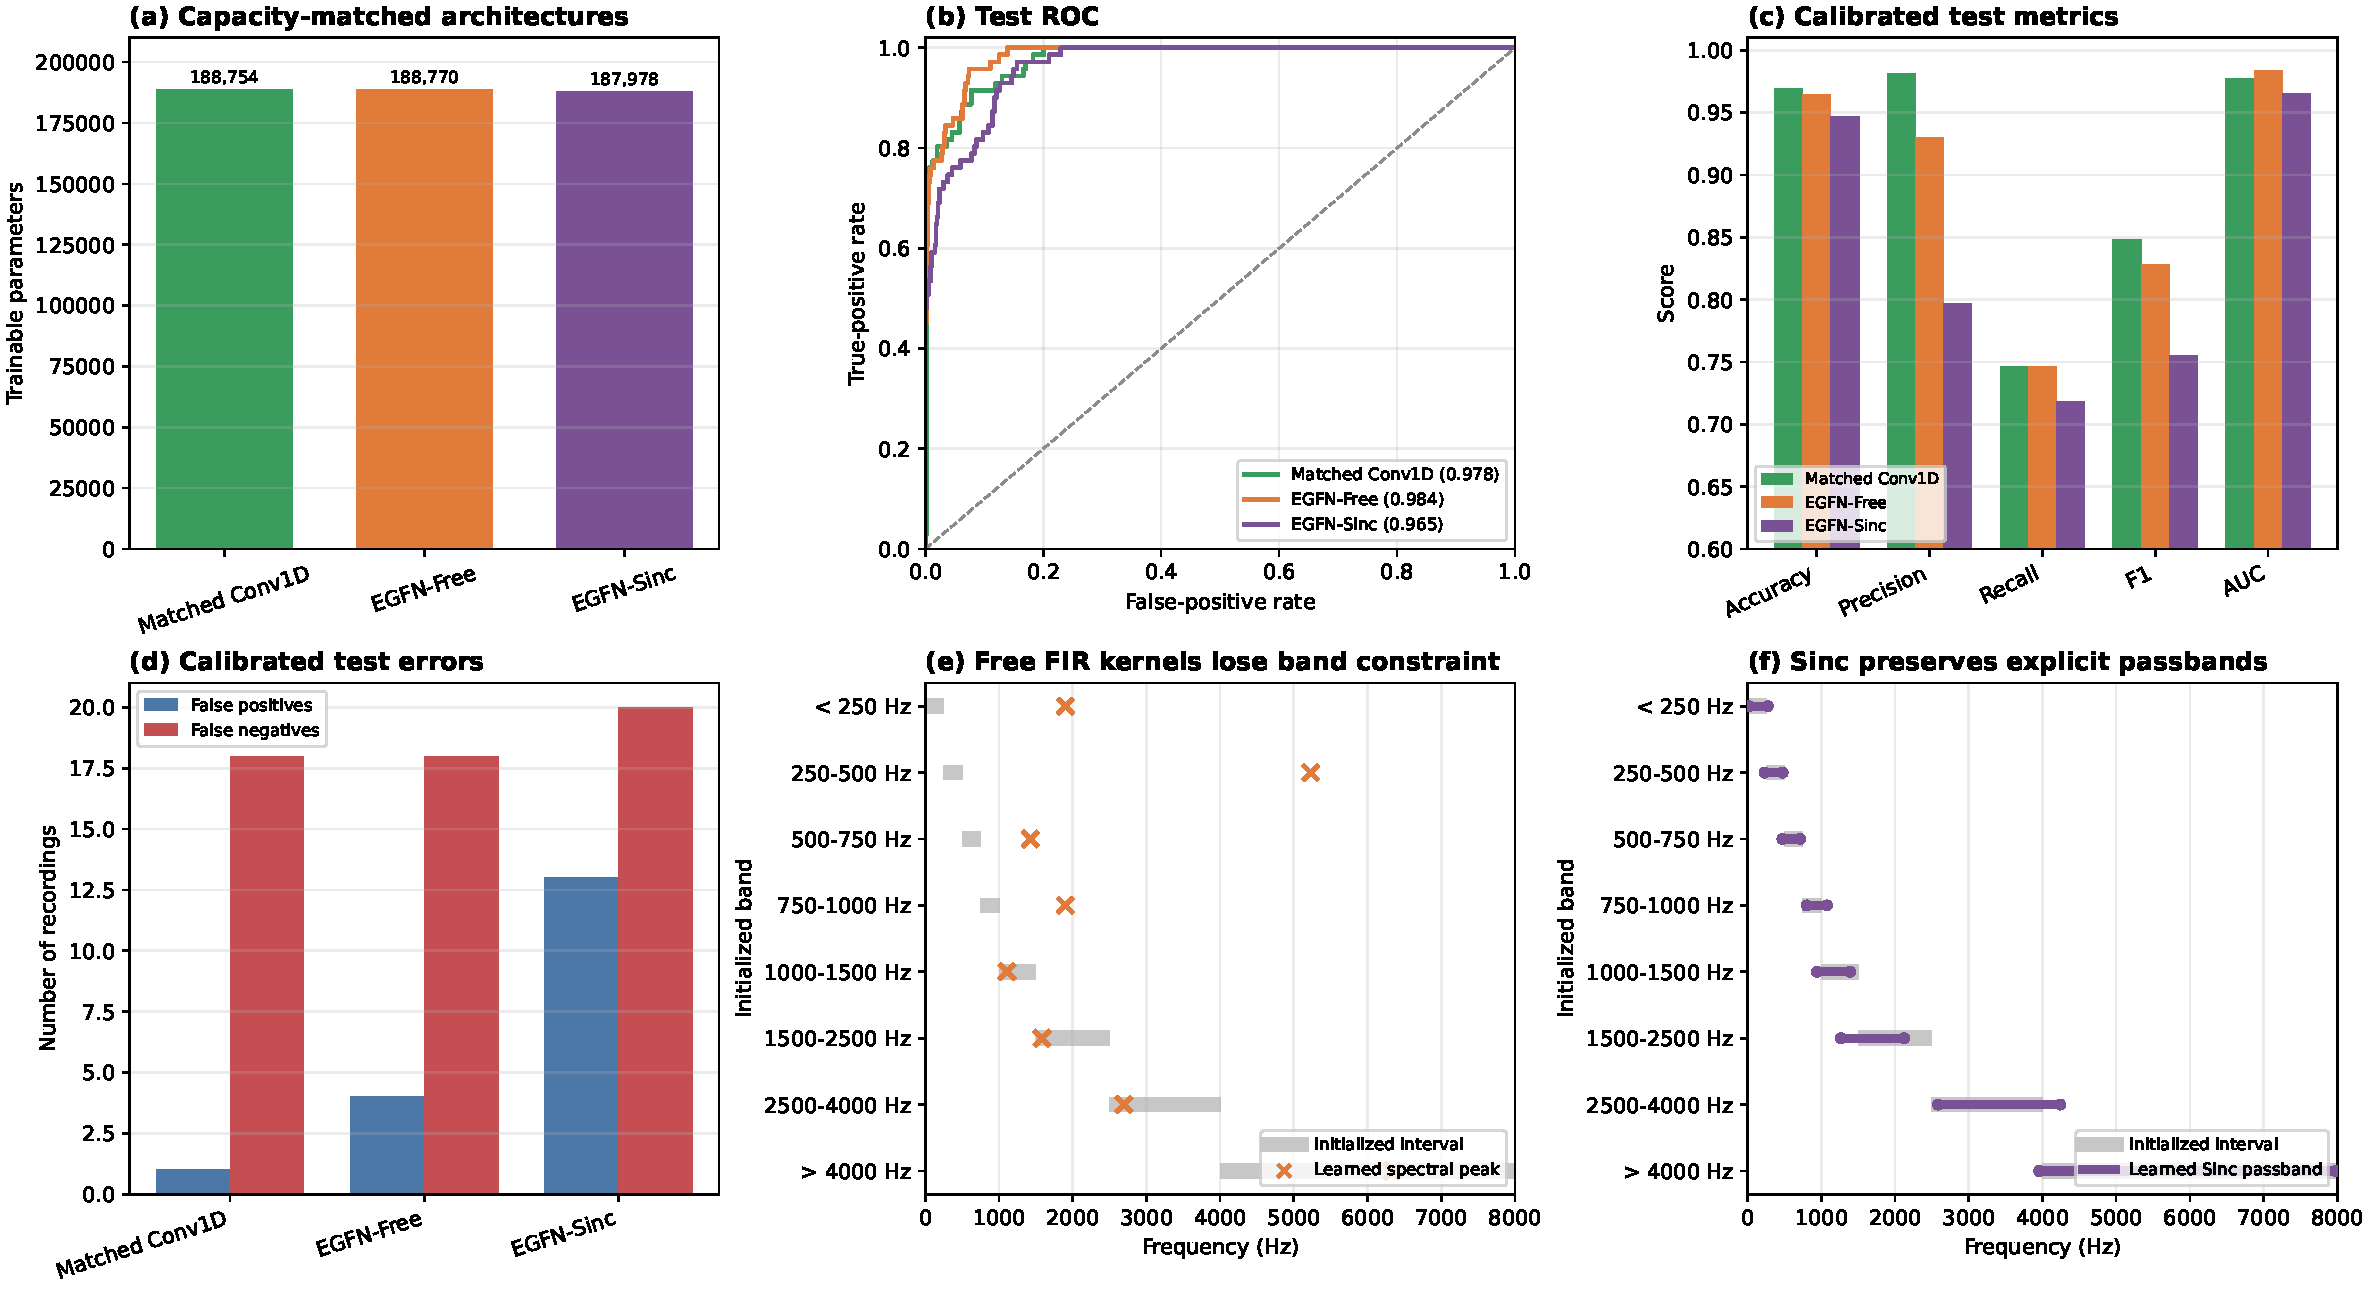
\includegraphics[width=0.98\textwidth]{fig10_mimii_v2.pdf}
\caption{Capacity-matched V2 screening experiment on seed 42. Matched Conv1D
obtains the best calibrated F1; \egfn{}-Free obtains the best AUC; \egfn{}-Sinc
preserves explicit physical passbands but loses predictive performance.}
\label{fig:v2}
\end{figure*}
\FloatBarrier

\begin{table}[t]
\centering
\caption{V2 seed-42 calibrated test results.}
\label{tab:v2results}
\small
\begin{tabular}{@{}lccc@{}}
\toprule
Model & Accuracy & F1 & AUC \\
\midrule
Matched Conv1D & \textbf{0.970} & \textbf{0.848} & 0.978 \\
\egfn{}-Free & 0.965 & 0.828 & \textbf{0.984} \\
\egfn{}-Sinc & 0.947 & 0.756 & 0.965 \\
\bottomrule
\end{tabular}
\end{table}

The control changes the interpretation of V1. Once temporal capacity is
matched, the unconstrained Conv1D frontend produces the best thresholded F1,
while free \egfn{} retains a small AUC advantage. There is no uniform winner.
The Sinc variant answers the technical criticism that free kernels can become
ordinary convolutions: its filters remain explicit band-pass systems, but this
constraint incurs a substantial performance cost in the seed-42 screening run.
Because V2 contains one seed, it is evidence about this controlled run rather
than a statistically definitive ordering.

\section{Discussion}

\subsection{Answer to the central question}

The experiments answer the original question in two parts. First, classical
filtering principles can be embedded in a differentiable network, and explicit
per-band energy can modulate neural activations. The sinusoidal sweep verifies
the mechanism directly. It does not establish that learned gating improves
prediction over the same filter bank with identity modulation. Second, the
mechanism does not automatically produce better generalization or efficiency
than Conv1D. Task difficulty, temporal modeling, filter freedom, model capacity,
and threshold selection all matter.

\subsection{Observability is not physical interpretation}

\egfn{} provides \emph{observability} by exposing filters, energy, and gates.
Physical \emph{interpretability} requires an additional link between those
variables and a verified mechanism. In free mode, channel names cease to be
physically guaranteed. In Sinc mode, cutoff frequencies remain meaningful, but
a high gate still does not establish causal relevance. Per-band ablations and
mechanical ground truth are needed to make that stronger claim.

\subsection{Industrial diagnostic hypothesis}

The MIMII results motivate, but do not demonstrate, diagnostic utility. The
dataset labels used here distinguish normal from anomalous recordings; they do
not connect each example to a verified fault mechanism or characteristic fault
frequency. A future study could test whether energy or modulation changes align
with rotational imbalance, misalignment harmonics, bearing frequencies,
cavitation, leakage, friction, or wear when speed, load, and fault annotations
are available. Until that experiment is performed, industrial diagnosis is a
hypothesis rather than a conclusion of this work.

\subsection{Limitations}

\begin{itemize}
  \item The synthetic experiments simplify real acoustics and room response.
  \item FSDD has only six speakers; speaker-disjoint estimates are therefore
        sensitive to speaker selection.
  \item Speech Commands compares different parameter counts.
  \item The MIMII multiseed experiment uses only three seeds.
  \item V2 is a one-seed screening control and needs paired repetition.
  \item No matched filter-bank-without-gating ablation is reported, so the
        predictive contribution of the gate remains unidentified.
  \item SincNet and LEAF are discussed but not implemented as direct baselines.
  \item Mean gates are not a causal explanation and did not become hard sparse.
  \item Only MIMII valves were used, without sample-level physical fault labels.
\end{itemize}

\subsection{Future work}

The first follow-up is a paired ablation with an identical temporal head:
free-filter bank without gating versus free-filter \egfn{}, and Sinc frontend
without gating versus Sinc \egfn{}. Direct SincNet and LEAF baselines should
then locate the architecture relative to established learnable frontends. These
comparisons require paired multiseed repetition, latency and parameter counts,
and threshold-free as well as operational metrics. Industrial validation should
use datasets with machine type, speed, load, and verified fault mechanism so
that learned bands can be compared against known physical frequencies.

\section{Conclusion}

Under capacity matching, Conv1D equaled or exceeded \egfn{} on the operational
F1 metric; free-filter \egfn{} retained only a small ROC--AUC advantage in one
seed-42 configuration. No general performance or efficiency advantage was
established, and the contribution of gating itself remains unmeasured. The
demonstrated contribution is instead a frequency-structured processing path in
which band responses, energy, and learned modulation can be inspected. Free FIR
filters were flexible but weakened physical meaning, while Sinc parameterization
restored explicit passbands at a predictive cost in the controlled screening
run. The project therefore contributes a tested architecture, a reproducible
experimental progression, and a clear account of where the original hypothesis
succeeded, failed, and remains open.

\begin{quote}
\egfn{} should presently be viewed not as a replacement for Conv1D, but as a
research architecture for investigating frequency-dependent representation,
adaptive modulation, and physically constrained filtering in neural audio
models.
\end{quote}

Its most compelling future role is in condition monitoring, where a model may
be valuable not only because it detects a fault, but because its internal
frequency variables can be compared with the physics of the machine.

\section*{Reproducibility Statement}

All figures in this report are generated from saved checkpoints, histories,
test diagnostics, and threshold reports in the project repository. Figure
scripts are stored under \texttt{scripts/plot\_*.py}. Data splits, seed values,
parameter counts, and validation-selected thresholds are exported as CSV files.
The project uses Python, PyTorch, torchaudio, NumPy, SciPy, scikit-learn, and
Matplotlib. No test-set threshold optimization is used.

\small
\begin{thebibliography}{9}

\bibitem{vaswani2017attention}
A. Vaswani, N. Shazeer, N. Parmar, J. Uszkoreit, L. Jones, A. N. Gomez,
L. Kaiser, and I. Polosukhin,
``Attention Is All You Need,'' in \emph{Advances in Neural Information
Processing Systems}, 2017. arXiv:1706.03762.

\bibitem{lecun2015deep}
Y. LeCun, Y. Bengio, and G. Hinton,
``Deep learning,'' \emph{Nature}, vol. 521, pp. 436--444, 2015.

\bibitem{ravanelli2018sincnet}
M. Ravanelli and Y. Bengio,
``Speaker Recognition from Raw Waveform with SincNet,''
arXiv:1808.00158, 2018.

\bibitem{zeghidour2021leaf}
N. Zeghidour, O. Teboul, F. de Chaumont Quitry, and M. Tagliasacchi,
``LEAF: A Learnable Frontend for Audio Classification,''
in \emph{International Conference on Learning Representations}, 2021.

\bibitem{warden2018speech}
P. Warden,
``Speech Commands: A Dataset for Limited-Vocabulary Speech Recognition,''
arXiv:1804.03209, 2018.

\bibitem{jackson2016fsdd}
Z. Jackson et al.,
``Free Spoken Digit Dataset,'' 2016--2020. [Online]. Available:
\url{https://github.com/Jakobovski/free-spoken-digit-dataset}

\bibitem{purohit2019mimii}
H. Purohit, R. Tanabe, K. Ichige, T. Endo, Y. Nikaido, K. Suefusa, and
Y. Kawaguchi,
``MIMII Dataset: Sound Dataset for Malfunctioning Industrial Machine
Investigation and Inspection,'' arXiv:1909.09347, 2019.

\bibitem{paszke2019pytorch}
A. Paszke et al.,
``PyTorch: An Imperative Style, High-Performance Deep Learning Library,''
in \emph{Advances in Neural Information Processing Systems}, 2019.

\end{thebibliography}

\end{document}
